% !TeX spellcheck = en_EN-English

\section{Embedding of Patient}
\label{embeddingImple}

The first sub-task in predicting a patient’s future costs is to embed each patient record into a numerical vector that can be interpreted by a neural network. For each patient record, four types of information are embedded. The first and easiest to implement is the timestamp, which is computed using numerical and date values. The other three, which are more complex, are the diagnosis, medical procedure, and prescribed drug.

\subsection{Timestamp}
\label{timespampImple}

To compute the timestamp, we first gathered all records for a single patient and identified the one with the earliest date. This record served as a pivot for calculating all timestamps for the patient. To compute the timestamp for this initial record, we took the patient's age in years, added half a year, and then multiplied by 365 to obtain an approximate age in days, which served as the timestamp. We added half a year to improve the approximation, as we only have the age in years and do not know whether the patient's birthday occurred one or eleven months ago; however, we assumed it to be on average six months, or half a year. For all subsequent records, we calculated the difference in days between the record date and the date of the first record, and then added this difference to the timestamp from the first record to create the timestamp for each subsequent record.

\subsection{Diagnosis embedding}

As discussed in Sec. \ref{diagEmb}, the embedding of diagnoses is based on the MKCH-10-SK (ICD-10-CM) code of the disease. We split this code into three parts, embed each part independently, and finally concatenate the results.
\\

To embed the main category, we generated a vector containing random numbers using a uniform distribution for each letter of the English alphabet. We chose to sample these random numbers from the interval [-0.5, 0.5]. This interval was chosen mostly arbitrarily, as we planned to pass the resulting embedding into a normalization function once it was complete.
\\

For the subcategory and details, we linearly assigned a value to each possible two-digit code. We chose the interval for these values to be [-0.5, 0.5], meaning subcategory 00 would get -0.5, category 50 would get 0, and category 99 would get 0.5. This interval was chosen so that each dimension of this embedding would have the same mean and standard deviation as each dimension of the main category. As a result, they also have, on average, the same distance per dimension. This means that each position of each part of the embedding should contribute to the total distance with the same weight.
\\

The most important part was to assign lengths to the vector of each part in a way that would encode their importance. The main category, the most important part, got a vector of length 28, the subcategory part got length 7, and finally, the details got length 3.
\\

A showcase of the resulting embedding can be seen in Fig. \ref{fig:diag_emb_show}, where each part is highlighted by a different color and all values are rounded to two decimals.

\begin{figure}[!h]
	\centering
	
	% TODO image needs update after change of lengths of each embeddings
	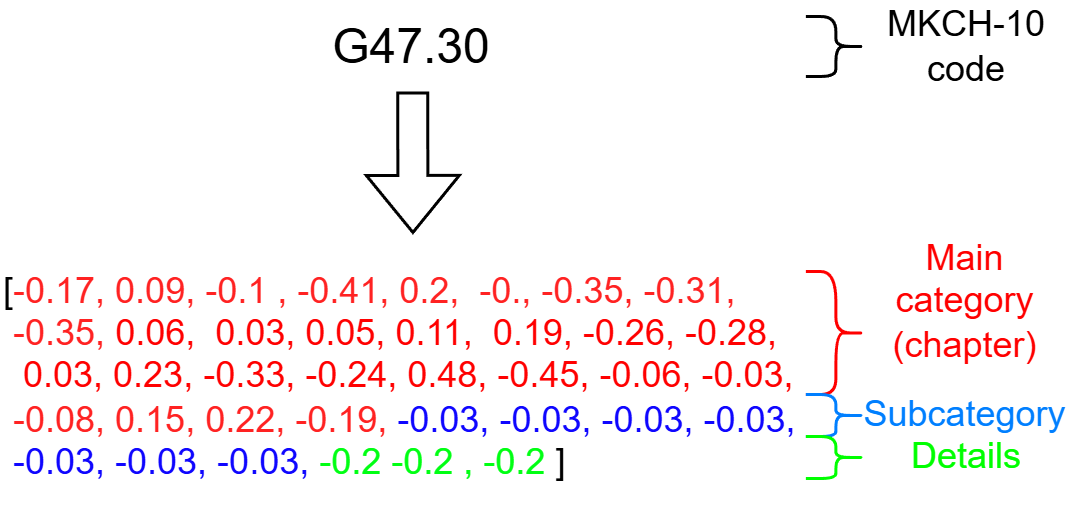
\includegraphics[width=0.8\textwidth]{images/diagnosis_embed_showcase.png} 
	
	\caption{Showcase of resulting embedding of specific diagnosis (rounded to two decimal places).}
	\label{fig:diag_emb_show}
\end{figure} 


\subsection{Drug embedding}

The embedding for drugs was performed similarly to the diagnosis embedding: each level was embedded separately, and the final embedding was created by concatenating them. For drug codes, each level was embedded using a random vector sampled from a uniform distribution over the interval [-0.5, 0.5]. We chose random vectors because none of the ATC levels contain internal subgroupings analogous to the hierarchical subgroups in diagnosis codes (see Sec. \ref{mkch_subdiv}). To encode the importance of each level, we again varied the vector lengths, with higher levels (e.g., anatomical groups) assigned shorter vectors. The specific vector lengths for each level are provided in Tab. \ref{tab:drug_lev_len}, resulting in a total embedding length identical to the diagnosis embedding. If a code is incomplete (i.e., missing higher levels), the missing parts are replaced with zero vectors, which act as neutral elements in the embedding space.
\\

\begin{table}[!h]
	\centering
	\begin{tabular}{|l|l|}
		\hline
		Level  & Length \\ \hline
		1 & 21 \\ \hline
		2 & 9 \\ \hline
		3 & 5 \\ \hline
		4 & 2 \\ \hline
		5 & 1 \\ \hline
	\end{tabular}
	\caption{Lengths of random vectors assigned to each information level of ATC code.}
	\label{tab:drug_lev_len}
\end{table}  

With this embedding, we should obtain codes whose similarity is more dependent on whether the lower, more important levels match than the higher ones.

\subsection{Medical procedure embedding}

Embedding of medical procedures was straightforward since we used an already trained model.
\\

As discussed in Sec. \ref{procedureEmb}, for the LLM we chose the LaBSE model. It is a model developed by Google to encode text into high-dimensional vectors. This model was trained on 109 languages, including Slovak. Using this model was straightforward, as we just had to input the complete description of the procedure to receive a 768-dimensional dense encoding of it. After computing all embeddings, we performed principal component analysis (PCA) to reduce the dimensionality of this embedding while maintaining most of the variance, or in other words, most of the information stored inside it.
\\

We also tried a different approach using a Word2vec model trained specifically for the Slovak language. More specifically, we used the word2vec-sk model made by the company Essential Data \cite{w2v}. This model was trained on a corpus containing around 110 million words. We chose the version of the model trained using the CBOW approach. Since this model is trained to embed words and not text, we first split the description of the procedure into words and lemmatized those words, in other words, changed them into their base form. Then, using the Word2vec model, we embedded each word into a dense 200-dimensional vector separately and finally created the description embedding as an average of the embeddings of all words in it.
\\

We expected that the LaBSE model would produce better results compared to standard text embedding models trained solely on the Slovak language, since the LaBSE model is trained by comparing embeddings not only to similar sentences in Slovak but also to their translations in other languages. This could mitigate the relatively small amount of Slovak language data compared to other, more commonly used languages. Additionally, this model could recognize domain-specific words, in our case medical terms, which are often left in a foreign language and would most likely not be found in a Slovak-only corpus.
\\

Finally, we create the record embedding by concatenating all four parts. Since we have two separate datasets, one for prescribed drugs and one for medical procedures, we always have only three out of four pieces of information available for each record. Since timestamp and diagnosis are always available, we substitute the missing part with a vector of zeros of appropriate length, which is the most neutral embedding since we centered both medical procedure and drug prescription embeddings around zero.
